\documentclass{standalone}
\usepackage{ tikz }
\usepackage{ xparse }
\usepackage{../../../macros}

\begin{document}
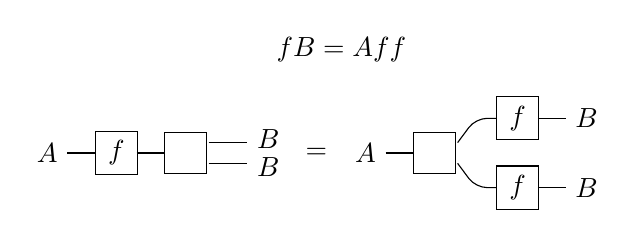
\begin{tikzpicture}[yscale=-1,x=1em,y=1.25em]

    \node [anchor=east] at (-0.5,0) {$A$};
    \node [anchor=west] at (6,-0.4) {$B$};
    \node [anchor=west] at (6,0.4) {$B$};
    
    \draw (-0.5,0) -- (0.5,0);
    \node[draw, minimum height = 1.5em, minimum width = 1.5em, anchor = west] at (0.5,0){$f$};
    \draw (2,0) -- (3,0);
    \node[draw, minimum height = 1.5em, minimum width = 1.5em, anchor = west] at (3,0){$\ccopy{}$};
    \draw [rounded corners] (4.6,-0.3) -- (6,-0.3);
    \draw [rounded corners] (4.6,0.3) -- (6,0.3);

    \node at (8.5,0) {$=$};
    \node at (9.4,-3) {$f \seq \ccopy{B} = \ccopy{A} \seq f \tensor f$};

    \node [anchor=east] at (11,0) {$A$};
    \node [anchor=west] at (17.5,-1) {$B$};
    \node [anchor=west] at (17.5,1) {$B$};
    
    \draw (11,0) -- (12,0);
    \node[draw, minimum height = 1.5em, minimum width = 1.5em, anchor = west] at (12,0){$\ccopy{}$};
    \draw [rounded corners] (13.6,-0.3) -- (14.25, -1) -- (15,-1);
    \draw [rounded corners] (13.6,0.3) -- (14.25,1) -- (15,1);

    \node[draw, minimum height = 1.5em, minimum width = 1.5em, anchor = west] at (15,-1){$f$};
    \node[draw, minimum height = 1.5em, minimum width = 1.5em, anchor = west] at (15,1){$f$};

    \draw (16.5,-1) -- (17.5,-1);
    \draw (16.5,1) -- (17.5,1);

\end{tikzpicture}
\end{document}